\documentclass[border=4pt]{standalone}
\usepackage{tikz}
\usetikzlibrary{shapes.symbols,positioning}

\begin{document}
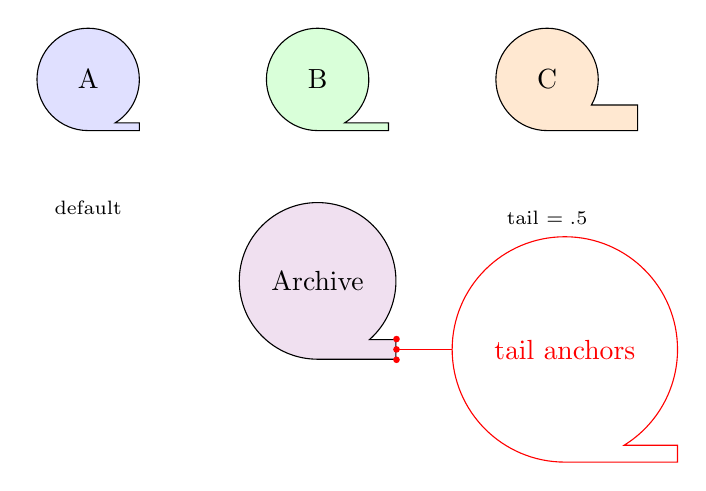
\begin{tikzpicture}[
  every node/.style={magnetic tape,draw,minimum size=13mm,align=center},
  node distance=9mm and 16mm
]
  \node[fill=blue!12] (default) {A};
  \node[magnetic tape tail extend=2.5mm,fill=green!15,right=of default] (extended) {B};
  \node[magnetic tape tail=.5,magnetic tape tail extend=5mm,
    fill=orange!18,right=of extended] (thick) {C};

  \node[shape=magnetic tape,magnetic tape tail=.25,minimum width=18mm,
    fill=violet!12,below=of extended] (wide) {Archive};
  \fill[red] (wide.tail north east) circle (1.2pt);
  \fill[red] (wide.tail east) circle (1.2pt);
  \fill[red] (wide.tail south east) circle (1.2pt);
  \draw[red,thin] (wide.tail east) -- ++(7mm,0) node[right]{tail anchors};

  \node[below=2mm of default.south,font=\scriptsize,draw=none,minimum size=0pt]
    {default};
  \node[below=2mm of thick.south,font=\scriptsize,draw=none,minimum size=0pt]
    {tail $=.5$};
\end{tikzpicture}
\end{document}
